\documentclass[10pt,a4paper, twocolumn]{report}
\usepackage[utf8]{inputenc} 
\usepackage[spanish]{babel}
\usepackage{amsmath}
\usepackage{amsfonts}
\usepackage{amssymb}
\usepackage{graphicx}
\usepackage{multirow}
\author{Antonio Molina García-Retamero}
\title{Optimización de redes neuronales mediante métodos bioinspirados}
\makeindex
\begin{document}
\onecolumn
\maketitle
\pagebreak
\tableofcontents
\pagebreak
\twocolumn

\chapter{Introduction}
\section{Notas}
\begin{itemize}
	\item En Haykin, en el capítulo 10, habla de los modelos teóricos de información. Hay cosas chulas, con las que puedo apoyar la metaplasticidad
	 \item Además, en ese mismo capítulo, trata también de las gausianas sus propiedades. También la relación con la entropía del conocimiento a priori de los parámetros de la gausiana.
	 \item Entre las diferentes técnicas de entrenamiento de redes RBF, la técnica de las k-medias puede ser sustituida por otras con tal de evitar el tiempo de cómputo. Sin embargo, a partir de estas k-medias podemos acelerar el proceso de aprendizaje en el BP. Tal vez así conseguimos mejores resultado en tiempo similares.
\end{itemize}

\section{Motivaciones}

\section{La metaplasticidad en redes biológicas}

\section{Metaplasticidad en redes neuronales artificiales}
\section{Trabajos previos}
El término metaplasticidad aplicado a redes artificiales fué acuñado por el doctor Andina en (ref). Andina definió la metaplasticidad en redes neuronales artificales como:
\begin{quote}
During the AMMLP training phase, the matrix weight W that models the synaptic strength of its artificial neurons is updated according to the probability of the input patterns and therefore of the corresponding synaptic activations
\end{quote}
\chapter{Metaplasticidad en Redes Neuronales con Función de Base Radial (RBFNN)}
\section{Estudio previo}
\subsection{Investigación del estado del arte y posibles vías de actuación}

\subsection{Estudio del trabajo sobre la metaplasticidad en redes neuronales}
\subsection{Implementación y estudio de la metaplasticidad en MLPs}
\section{La naturaleza stadística del proceso de aprendizaje}
Aquí me gustaría esponer una base sobre la que sustentar la idea de mejorar el proceso de aprendizaje en RBFNN implementado el concepto de metaplasticidad
\section{Refuerzo de casos menos frecuentes}
De acuerdo a lo descrito anteriormente, podemos considerar el proceso de metaplasticidad neuronal en redes artificiales como el refuerzo del aprendizaje en base a la probabilidad de pertenecencia a una clase de una muestra concreta. Así, para un caso típico (sus características son "frecuentes" en una clase, su influencia en el peso "influencia psinactica" será menor que para un caso "atípico" de la clase.
La idea intuitiva   
\section{Mi intuición de metaplasticidad en RBFNN}
En base a los trabajos previos, la idea de servirnos de la naturaleza de los datos de nuestro entrenamiento para hacernos una idea a priori de cuan significativa es una muestra y actuar ponderando esa "conexión sináptica" concreta parece encajar de forma especial en el concepto de RBFNN debido a la naturaleza de las Funciones de Base Radial. Quiero decir, las Funciones de Base Radial nos proporcionan una transformación no lineal que nos permite encontrar un hiperplano que en algún espacio multidimensional nuestros datos serán separables. El modelo de las RBFNN, como ya hemos comentado, se sirven de un modelo con la forma $f(x)=\sum w \phi(x)$ donde $\phi(x)$ es un función de base radial. Este tipo de funciones pueden ser muy variadas y se ha experimentado con multitud de ideas alrededor de esto sin embargo en los casos más habituales se utiliza una función gausiana en donde tenemos que inferir tanto la media como los centroides para cada una de las funciones en nuestro training set. De esto se deriva un entrenamiento de dos fases en el que en la primera fase inferimos los datos necesarios para calcular la activación de la capa oculta para hacer luego encontrar los parámetros para la transformación lineal sobre la salida de esta capa en una segunda fase de entrenamiento.

Aquí es donde pretendo encontrar y probar diferentes formas de optimizar la segunda fase de entrenamiento sirviéndonos del estudio estádico que implica la primera fase. Esto es, Cuando en la primera fase de entrenamiento buscamos los centros para nuestras funciones de activación obtenemos información relevante que podemos utilizar para estimar, como hablábamos antes, como considerar una probabilidad de pertenencia a una clase si consideramos el centroide como una clase, etc... Multitud de ideas se pueden considerar y en última instancia lo que se estaría haciendo sería entremezclar de diferentes formas el proceso de aprendizaje no supervisado a priori para influir en el proceso de aprendizaje supervisado de la segunda fase.

\section{Entrenamiento}
Explico las bases y explico mis intuiciones
\chapter{Implementación}
Tendría que encontrar el sitio donde poner qué se ha implementado y por qué
\section{Metodología de desarrollo}
Aquí comento que he realizado la implementación siguiendo el paradigma TDD para la implementación de las redes.
\section{Lenguaje y herramientas}
\section{Implementación de las redes}
\section{Pruebas y métricas de rendimiento}
Dado que por medio de este trabajo se pretende la demostración de la mejora propuesta sobre las RBFNN, estableceré una serie de pruebas que pretenderán poner a prueba las diferentes implementaciones de las redes para resolver problemas típicos de aprendizaje máquina.
En secciones anteriores hemos comentado la problemática y las diferentes alternativas propuestas para entrenar las RBFNN. La batería de pruebas es la parte probablemente más crítica del proyecto y con especial esmero he diseñado un conjunto de pruebas que pretende ser exhaustivo y con el que pretendo primero valorar el comportamiento de las soluciones típicas existentes y las mejoras propuestas en esta investigación.

De entre los escenarios típicos del aprendizaje máquina podemos hacer dos grandes grupos: tal y clasificación. Para este proyecto he seguido la estrategia de construir, para sendos tipos de problemas, sets de datos aleatorios cuyos parámetros intrínsecos puedan ser manipulados fácilmente permitiendo generar de forma sencilla tantos escenarios como se crean apropiados para los diferentes test. En busca de evitar el "data snooping" y una vez determinadas las configuraciones para los que los diferentes tipos de redes tienen comportamientos interesantes, las redes serán testeados sobre sets de datos estándares en la investigación sobre aprendizaje máquina.

\begin{itemize}
	\item Reconocimiento de patrones
	\begin{itemize}
		\item Onda compuesta aleatoria
		\item Otra idea que se me ocurra
	\end{itemize}
	\item Clasificación
	\begin{itemize}
		\item Clasificación sobre datos aleatorios artificiales
		\item Clasificación sobre datos reales
	\end{itemize}
\end{itemize} 
En las siguientes secciones trataré de clarificar todo esto para cada tipo de pruebas. Explicaré las cosas fundamentales de la implementación tratando de no perder al lector en el código pero dándo una visión clara y precisa de lo que se desea poner a prueba con cada test. Sin embargo, antes de entrar en detalle sobre la construcción de los conjuntos de datos me gustaría dejar patente el guión básico que sigo a la hora de diseñar las prubas.

Anteriormente hemos discutido las fases del entrenamiento de redes RBFNN y de las soluciones típicas. Además discutimos acerca de como podemos implementar la intuición de la metaplasticidad en la fase supervisada a partir de la información estadística que supone el aprendizaje no supervisado de la primera parte del entrenamiento en busca de los parámetros de las funciones de base radial. 

Con todo esto, una primera batería de test tratará de determinar en qué condiciones, el cálculo de la pseudoinversa deja de resultar rentable en términos de coste computacional con respecto a al descenso por gradiente. Este coste computacional es directamente proporcional al tamaño del set de datos, con lo que esta prueba nos dará una estimación de cuan grande ha de ser al menos nuestro conjunto de datos para que resulte rentable la aproximación del descenso por gradiente que es necesario para la implementación de la intuición de metaplasticidad aquí propuesta.

A continuación, someteremos a una batería exahustiva de test generados artificialmente y sobre los que variaré los parámetros de los diferentes tipos de redes y de los propios conjuntos de datos en busca de las condiciones en que cada tipo de RBFNNs de los propuestos ofrece un comportamiento mejor que el resto. Con esto podremos determinar si existen condiciones en las que, en efecto, la propuesta de metaplasticidad supone una mejora sobre las aproximaciones existentes.

Por último, se realizarán pruebas sobre sets de datos conocidos y ampliamente utilizados en el campo del aprendizaje máquina. Con esto se pretende evitar la aparición de resultados inválidos por la propia intervención y manipulación de los parámetros y datos en busca de las condiciones en las que la esta implementación resulte mejor además de poder ofrecer comparativas que puedan ser reconocidas por quienes trabajan en otras propuestas sobre los mismos conjuntos de datos.

\subsection{Pruebas de clasificación}
Uno de los usos más habituales de las RBFNN es cuando tenemos que clasificar sobre un conjunto de datos cuyas clases no son linealmente separables. Anteriormente hablamos de
\begin{figure}[!h]{}
    \centering
    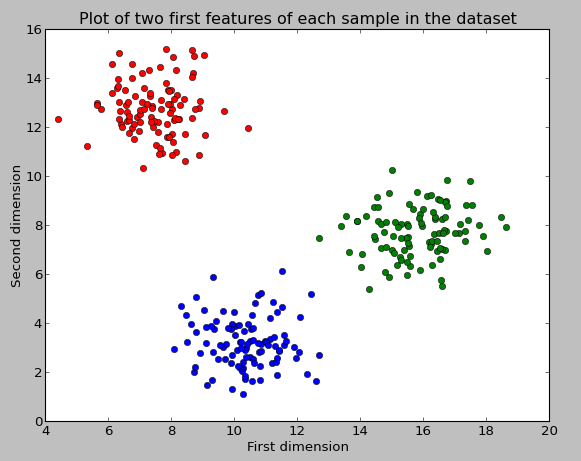
\includegraphics[width=0.4\textwidth]{img/clusteredData1.png}
    \label{fig:clusteredData1}
    \caption{Conjunto de datos con distribución normal}
\end{figure}
Ya que, a través de las RBFNN, obtenemos un modelo con la forma $f(x)=\sum w_{i}\phi(r)$ (que es caracterizado con funciones de base radial) podemos aproximar funciones complejas cuya salida sigue una distribución gaussiana (la más frecuente con mucha diferencia de entre las variables aleatorias que se dan en la naturaleza) con notable precisión. 
La figura \ref{fig:clusteredData1} es un ejemplo de datos generados con el generador de datos clusterizados que he implementado. Este recibe como parámetros básicos el número de centroides y el número de muestras y genera estos datos de forma aleatoria tomando como centro los k-centroides también tomados aleatoriamente. En las siguientes líneas introduciré esta clase sin entrar en excesivo detalle de la implementación pero sí tratando de aclarar las cuestiones que considero claves.

\subsubsection{Generación de datos aleatorios}
Para este tipo de test necesitamos generar datos que se distribuyan de forma normal alrededor de un centroide. Una distribución normal es aquella que cuya función de densidad de probabilidad queda definida por la media ($\mu$) y la desviación estándar ($\sigma$) del conjunto de datos ($x$) de la siguiente forma:
\begin{center}
$pdf(x,\mu,\sigma) = \frac{1}{ \sigma \sqrt{2 \pi}} e^{\left(-\frac{{\left(\mu - x\right)}^{2}}{2 \, \sigma^{2}}\right)}$
\end{center} 
Existen multitud de generadores aleatorios de este tipo de datos. En este caso utilizaré el propio de NumPy como muestro a continuación para generar las $n$ muestras por cada centroide ya que este definirá la media. La desviación estándard será proporcionada como parámetro en el constructor de la clase y nos permitirá jugar con la forma que adoptarán los datos generados.

\begin{figure}[!h]{}
    \centering
    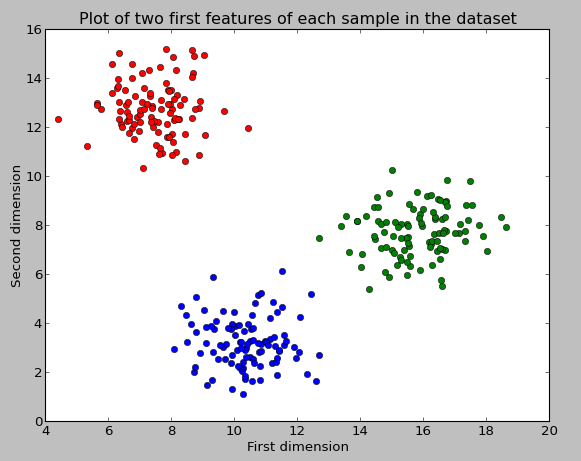
\includegraphics[width=0.4\textwidth]{img/clusteredData1.png}
    \label{fig:clusteredData1}
    \caption{Conjunto de datos con distribución normal}
\end{figure}
\section{Implementación básica de una RBF}

\section{Extendemos con centróides K-NN}

\chapter{Resultados}
\subsection{Pruebas de clasificación}
Ya hemos comentado anteriormente como he desarrollado el generador de datos aleatorios y como este evalúa el error del clasificador. En este proceso de evaluación consideraré una serie de conjuntos de datos con diferentes números de categorías que siguen una distribución normal en un número arbitrario de dimensiones. Sobre cada uno de estos conjuntos de datos evaluaré el funcionamiento de las distintan RBFNN estudiadas con diferente número de clústeres (neuronas con activación en base a una función de base radial en la primera capa de la red) evaluando tanto la clasificación (aciertos, fallos, falsos positivos, falsos negativos, preción y "recall") como los tiempos de entrenamiento.

\section{Comparativa de RBFNN con y sin metaplasticidad}
\section{Otros resultados de interés}

\onecolumn
\begin{center}\begin{tabular}{|c|c|c|c|c|c|c|}
	\hline
	\multicolumn{7}{|c|}{RBFNNs performance over n samples} \\
	\hline
	\multirow{2}{*}{nC} & \multicolumn{2}{|c|}{Random centroids} & \multicolumn{2}{|c|}{Knn} & \multicolumn{2}{|c|}{Metaplasticity} \\
	%\hline
	& Time & Accuracy & Time & Accuracy & Time & Accuracy \\
	\hline
	10 & 1 & 2 & 1 & 2 & 1 & 2 \\
	%\hline
	10 & 1 & 2 & 1 & 2 & 1 & 2 \\
	\hline
\end{tabular}\end{center}
\twocolumn

\end{document}
